% !TeX program = xelatex
\documentclass[UTF8,11pt,a4paper,fontset=none]{ctexart}
\usepackage[margin=23mm,headheight=16pt,footskip=13mm]{geometry}
\usepackage{fontspec}
\setmainfont{Noto Sans}
\setsansfont{Noto Sans}
\setmonofont[Scale=0.85]{DejaVu Sans Mono}
\setCJKmainfont{Noto Sans CJK TC}
\setCJKsansfont{Noto Sans CJK TC}
\setCJKmonofont{Noto Sans Mono CJK TC}
\usepackage{amsmath,graphicx,booktabs,tabularx,longtable,array,multirow}
\usepackage[table]{xcolor}
\usepackage{enumitem,fancyhdr,tcolorbox,caption,float,pdflscape}
\usepackage{hyperref,xurl}
\definecolor{navy}{HTML}{16324F}
\definecolor{teal}{HTML}{087F8C}
\definecolor{light}{HTML}{EFF5F8}
\definecolor{muted}{HTML}{536578}
\definecolor{amber}{HTML}{8F5310}
\hypersetup{unicode=true,colorlinks=true,linkcolor=navy,urlcolor=teal,citecolor=teal,
  pdftitle={Saccade v1 Dataflow：從影格輸入到追蹤結果},
  pdfauthor={Saccade v1 專案},pdfsubject={資料物件、GPU／CPU責任、跨幀排程、buffer交接與結果完成邊界}}
\urlstyle{same}
\renewcommand{\contentsname}{目錄}
\renewcommand{\refname}{證據與參考文件}
\ctexset{section={format=\Large\bfseries\sffamily\color{navy}},
  subsection={format=\large\bfseries\sffamily\color{navy}},
  subsubsection={format=\normalsize\bfseries\sffamily}}
\clubpenalty=10000
\widowpenalty=10000
\setlength{\parindent}{2em}
\setlength{\parskip}{0.35em}
\linespread{1.18}
\setlength{\emergencystretch}{1.5em}
\setlength{\tabcolsep}{5pt}
\renewcommand{\arraystretch}{1.30}
\newcolumntype{Y}{>{\raggedright\arraybackslash}X}
\newcolumntype{P}[1]{>{\raggedright\arraybackslash}p{#1}}
\setlist[itemize]{leftmargin=1.7em,itemsep=0.25em,topsep=0.35em}
\setlist[enumerate]{leftmargin=1.9em,itemsep=0.3em,topsep=0.35em}
\captionsetup{font=small,labelfont={bf,color=navy},skip=8pt}
\pagestyle{fancy}\fancyhf{}
\fancyhead[L]{\small\sffamily\color{muted}Saccade v1｜Dataflow}
\fancyhead[R]{\small\sffamily\color{muted}資料流圖解 v1.0}
\fancyfoot[L]{\scriptsize\color{muted}2026-11-12｜程式基準 3cbaa518f0dc}
\fancyfoot[R]{\small\thepage}
\renewcommand{\headrulewidth}{0.4pt}
\newtcolorbox{finding}[1][]{colback=light,colframe=teal,boxrule=0.7pt,
  arc=1mm,left=3mm,right=3mm,top=2mm,bottom=2mm,#1}
\newcommand{\code}[1]{\texttt{\detokenize{#1}}}
\newcommand{\status}[1]{\textbf{#1}}
\newcommand{\source}[1]{\par\noindent{\footnotesize\color{muted}來源：#1}\par}
\newcommand{\reportbase}{3cbaa518f0dc37d691404e95ed85c0109c81130d}
\begin{document}
\noindent{\small\sffamily\color{teal}SACCADE v1・DATAFLOW}\par
\vspace{4mm}
\noindent{\LARGE\bfseries\sffamily\color{navy}從影格輸入，到追蹤結果}\par
\vspace{3mm}
\noindent{\large\color{muted}影像、候選、運動與追蹤狀態，如何在 CPU／GPU 之間交接。}\par
\vspace{5mm}

\section{先追資料，再看每個階段}
一條追蹤流程不只是「先偵測，再追蹤」。真正需要接好的，是每份資料何時產生、由誰讀取、可以留多久，以及哪個時點之後能交給下一幀重用。

本文沿著一幀資料，說明目前 JPEG 主線：C++ host 讀取與排程，CUDA／TensorRT 在 GPU 處理影像、候選、運動與軌跡，最後回傳固定結果給 CPU。偵測器是每幀獨立的 spatial scan 模型；跨幀身份記憶由 tracker 保存，沒有額外 ReID 模型。\cite{session,model}

\begin{table}[H]
\caption{閱讀主線時，可以先記住這些資料物件}
\small
\begin{tabularx}{\textwidth}{@{}P{29mm}YY@{}}
\toprule
資料 & 它回答什麼 & 接下來交給誰 \\
\midrule
JPEG／RGB & 這一幀實際看到了什麼 & GPU 前處理與灰階分支 \\
Model tensor／raw & 模型在三個尺度輸出了什麼 & Producer 檢查與 F04 候選整理 \\
MotionImage（MI） & 供鏡頭運動估計使用的灰階影像 & M 上的 G1／NVOFA \\
Candidates（CS） & 哪些框保留、哪些框被 NMS 抑制 & 本幀 mask 與 F04b \\
MotionContext & 這次估計的全域位移是否有效 & GMC control／Kalman predict \\
Predicted prior & 軌跡在本幀預測的位置 & F04b 續追篩選與關聯 \\
TrackState／gray／mask & 下一幀要沿用哪個成功版本 & 下一次 G1 與追蹤更新 \\
ResultPacket & 此幀狀態、身份與座標 & CPU receive 與輸出定稿 \\
\bottomrule
\end{tabularx}
\end{table}

\begin{finding}
\textbf{本文採用的具體組合}\par
HR 1280×768、batch 1、FP16 tactics／FP32 模型 I/O，G1 NVOFA，CUDA Graph ON；MI／candidate／result slots=2／2／4。JPEG 主線需明確選 \code{hr-1280x768}；API／\code{track_sequence} 的初始 profile 仍是 640。NSA 與量測框維持 OFF。
\end{finding}

程式基準固定為 \code{3cbaa518f0dc}。本文描述這條 G1 主線；舊規劃文件中的 PCR／cuFFT 內容保留其歷史用途，現行 motion 以實作與 TRACKING §20 為準。\cite{session,flow}

\clearpage
\section{一幀影像分成兩條必要路徑}
原圖在 GPU 解碼後，一條分支產生模型輸入與候選，另一條產生獨立的運動影像。M 先處理運動與預測，等同幀候選準備好，再完成關聯和提交。

\begin{figure}[H]
\centering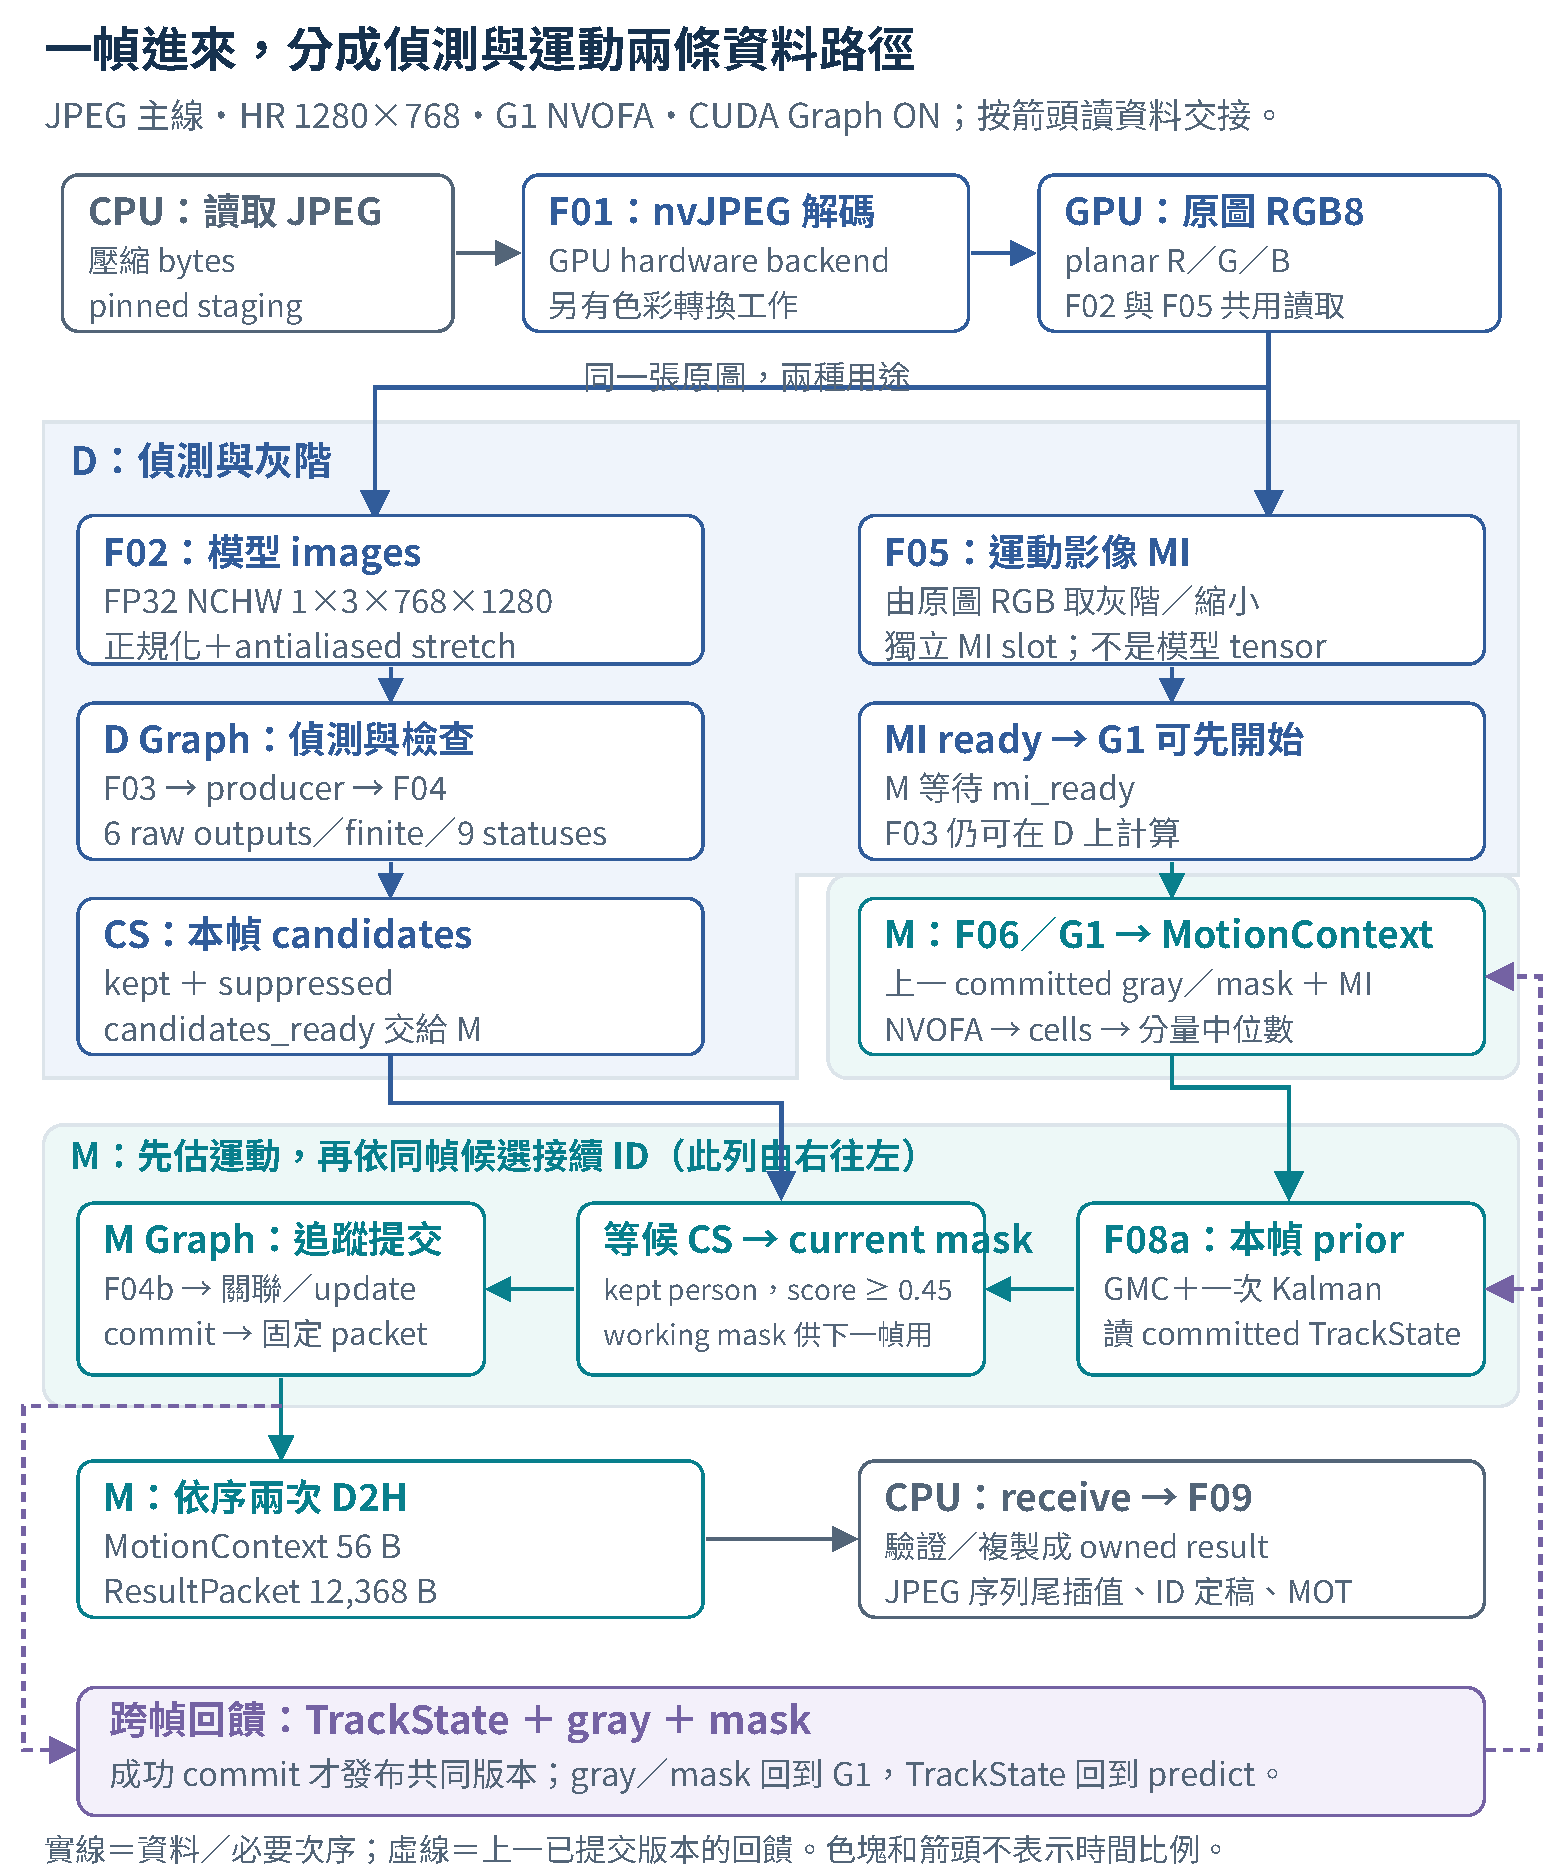
\includegraphics[width=\textwidth]{assets/flow.pdf}
\caption{資料與必要依賴。D／M 是執行責任；箭頭和區塊寬度不代表實測時間。}
\end{figure}

中間影像、模型 raw outputs、候選與 TrackState 都留在 GPU。Host 每幀收回的是 MotionContext 與固定封包，沒有為了 CPU 關聯把整張原圖或所有 raw tensors 下載。\cite{session,flow}

\clearpage
\section{偵測分支：從原圖，到可用的候選}
\subsection*{RGB 與模型 tensor 是不同物件}
F01 使用 nvJPEG 的 GPU decode 路徑產生原圖大小的 planar RGB8。F02 將 RGB 正規化並做 antialiased bilinear stretch，產生 FP32 NCHW。座標映射保留原圖尺寸；模型的框最後映回原圖像素座標。沒有 letterbox padding，也不做框座標 clipping。\cite{preprocess,post}

\begin{table}[H]
\caption{HR profile 的主要張量；大小是 payload，不是每幀傳輸或完整顯存}
\small
\begin{tabularx}{\textwidth}{@{}P{30mm}Yr@{}}
\toprule
資料 & 型別與形狀 & Payload \\
\midrule
原圖 RGB（1080p例） & uint8，3×1080×1920，planar & 6,220,800 B \\
模型 input & FP32，1×3×768×1280 & 11,796,480 B \\
P3 raw & cls 1×80×96×160；reg 1×4×96×160 & \multirow{3}{*}{合計 6,773,760 B} \\
P4 raw & cls 1×80×48×80；reg 1×4×48×80 & \\
P5 raw & cls 1×80×24×40；reg 1×4×24×40 & \\
Candidates & 64 B header＋最多 300×32 B rows & 9,664 B／slot \\
\bottomrule
\end{tabularx}
\end{table}

F03 使用 YOLO26m backbone／neck 與三尺度 scan head，共 20,160 個 positions、六個 FP32 raw outputs。Head 是 T=1 的空間掃描，每次從初始狀態開始；它沒有跨影格保存 Mamba hidden state。FP16 tactics 也不表示 input、raw、scan 或 tracker 狀態全部變成 FP16。\cite{model}

\subsection*{先檢查，再交付 kept／suppressed}
Producer 檢查 input／raw 是否有限，並彙整九個 plugin statuses。F04 以 score\ensuremath{\ge}0.001 形成全類別 top-300，再篩選 person，依 NMS IoU>0.5 區分 kept 與 suppressed；兩種結果留在同一候選契約內。\cite{post}

\begin{finding}
\textbf{被 NMS 抑制，不等於完全丟掉。}\par
F04b 等本幀 GMC control＋一次 predict 產生 prior 後，才決定哪些 suppressed 框可以補回。Kept 門檻為 0.05；suppressed 要 score\ensuremath{\ge}0.10、prior IoU\ensuremath{\ge}0.30，最多補 50 筆，只可續追、不能 birth。Kept 也仍受 birth 門檻與生命週期政策。
\end{finding}

\clearpage
\section{運動分支：讀前次成功版本，預測本幀位置}
F05 從原圖 RGB 另外產生 GRAYSCALE8 MotionImage。它有獨立 slot，並非模型 resize 後的 tensor，也不借用即將給下一張解碼覆寫的 RGB。

縮小倍率為 $s=\max(1,\lceil W/1920\rceil,\lceil H/1080\rceil)$；1080p 時 s=1，4K 時 s=2。MI 使用自己的 pitch；不能把影像有效 payload 當成實際配置大小。

\begin{table}[H]
\caption{G1 到追蹤預測的交接順序}
\small
\begin{tabularx}{\textwidth}{@{}P{30mm}YY@{}}
\toprule
步驟 & 讀取 & 產生／交付 \\
\midrule
G1 輸入 & 上次 committed gray＋本幀 MI & NVOFA 光流，grid 4、SLOW \\
Cells／中位數 & 光流、上次 committed mask & 8×8 cells；排除被 mask 標記的 cell \\
MotionContext & 剩餘 cell 的分量中位數 & 原圖單位 tx／ty 與有效狀態 \\
Gray 寫回 & 本幀 MI & working gray；完成後才發布 mi\_consumed \\
本幀 prior & 前次 committed TrackState＋GMC & 一次 Kalman predict；本幀預測位置 \\
本幀 mask & 本幀 kept person 候選 & working mask，供下次成功提交後使用 \\
\bottomrule
\end{tabularx}
\end{table}

G1 的位移是 translation-only。全域估計逐分量取中位數，再乘 s 回到原圖座標；可用 cells 少於 8 時回報 rejected，而不是把缺資料當成可靠運動。第一幀沒有前次參考，MotionContext 為 uninitialized。\cite{flow}

\textbf{遮罩的時間關係要分清楚。} G1 排除的是\textbf{上一個成功提交的 mask}；本幀 kept class 0、score\ensuremath{\ge}0.45 的框用來建立 working mask，按 cell 中心是否落框標記，提供給下一幀。不能用當幀尚未完成的偵測，假裝它在早先的 G1 階段已經可用。

\textbf{OFA 是 GPU 裡的固定功能引擎。} 周邊的灰階、copy、cell reduction、median 與 mask 仍有 CUDA 工作，\code{NvOFExecute} 仍是 host API；這條資料流不能理解成所有提交都在 device 自行發動。\cite{flow}

\clearpage
\section{n／n+1 可以交錯，狀態仍逐幀提交}
D 產生本幀 MI 後，G1／predict 可以與同幀的 F03 偵測重疊。D(n+1) 也可以往前做，與 M(n) 的追蹤尾端交錯；M(n+1) 的工作仍排在 M(n) 的 commit／packet／D2H 之後，只有成功 commit 才推進版本。

\begin{figure}[H]
\centering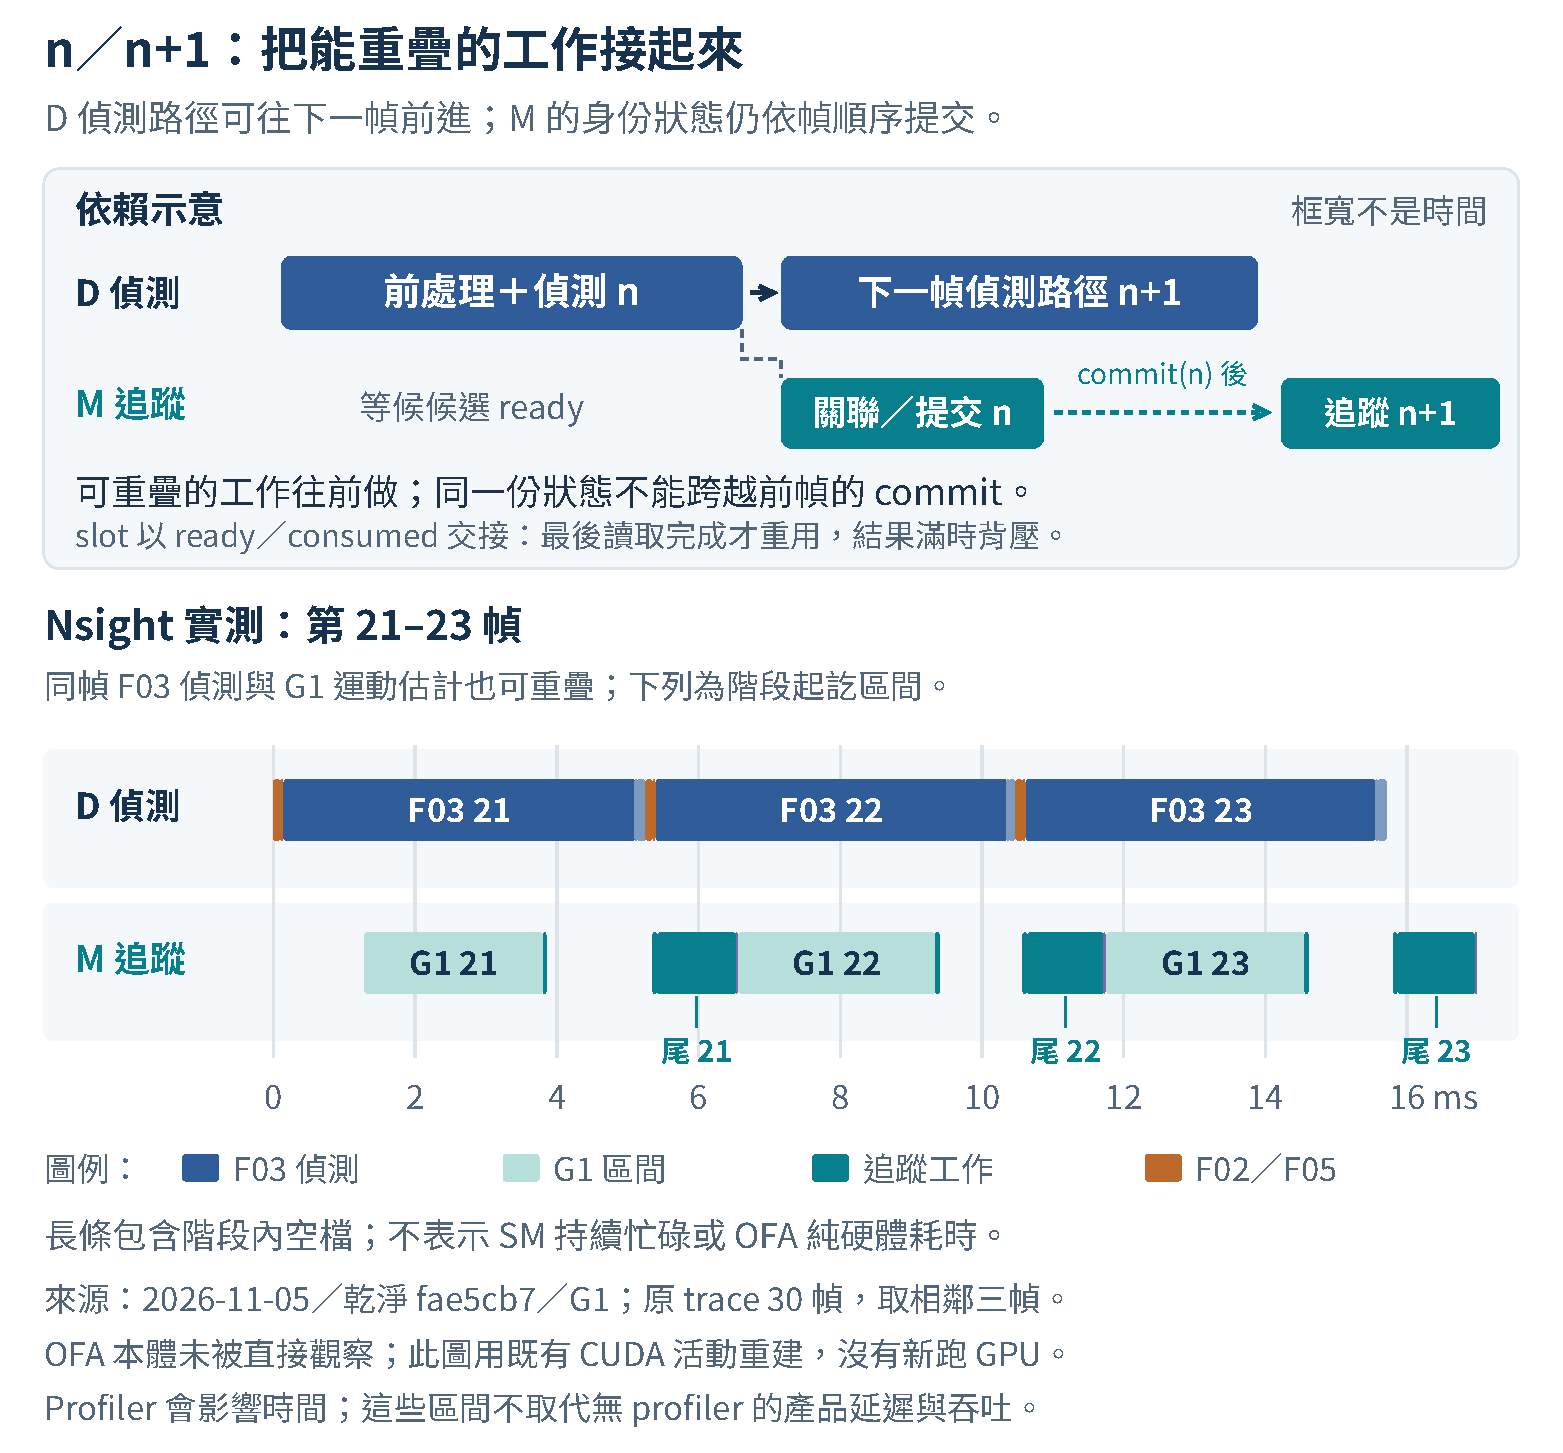
\includegraphics[width=\textwidth]{assets/schedule.pdf}
\caption{上方是依賴示意；下方是既有 G1 Nsight trace 的 JPEG 第 21–23 幀，只有下方橫軸是實測時間。}
\end{figure}

既有 30 幀 trace 排除初始化與首次 Execute 後，完整 F06 在 28／28 幀落入同幀 F03 區間；27／27 個相鄰穩態幀對有實際 CUDA 活動交集，平均 0.937 ms，主要是 F03(n+1) 與上一幀 mask／追蹤尾端。\cite{trace}

這是歷史乾淨 \code{fae5cb7}、driver 617.42 的 profiler 觀察，並非本次重新量測的產品延遲。長條包住階段空檔；OFA 本體沒有被直接觀察。實際活動聯集、階段包圍區間與端到端延遲各自保留口徑。

\clearpage
\section{Buffer 何時能交還給下一幀？}
Ready 代表資料已可讀；consumed 代表最後一次讀取結束、producer 可以重用。Header 的 frame／epoch 核對用來診斷身份，不能取代這些同步邊。

\begin{figure}[H]
\centering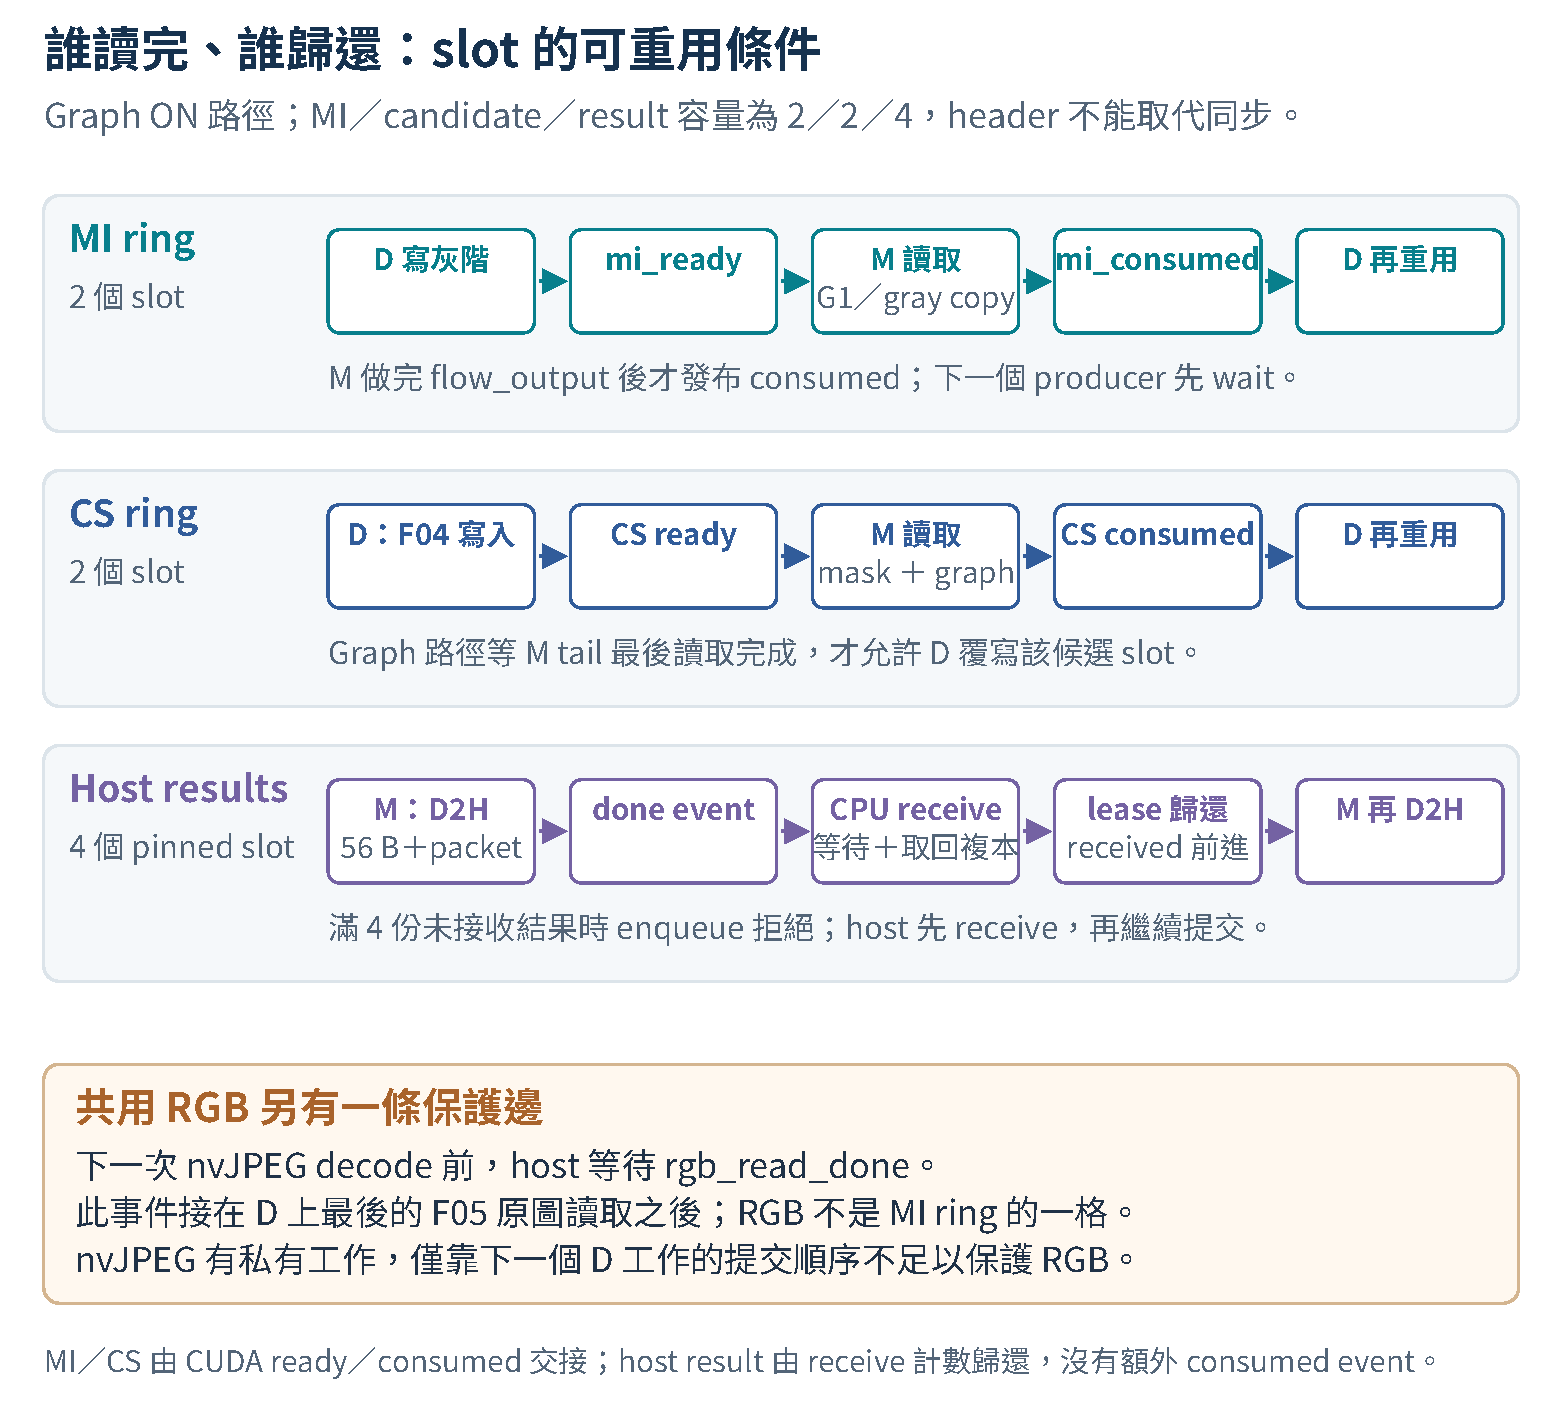
\includegraphics[width=\textwidth]{assets/leases.pdf}
\caption{Slot 的借出與歸還。MI／候選／結果 ring 與跨幀 state 雙版本是不同資源。}
\end{figure}

\textbf{MI 與候選分開歸還。} MI 在 flow\_output 完成本幀 gray 寫回後歸還；Graph 路徑的 CS 則在 M tail 結束後才發布 consumed。

\textbf{原圖 RGB 另有保護。} 下次 nvJPEG decode 前，host 等 rgb\_read\_done，確認 F02／F05 最後讀取結束；nvJPEG 私有 stream 不會自動排在 D 的前次工作後面。模型 input／raw／scratch 則由同一 D stream 的次序與固定地址契約保護。


Result ring 滿會在提交前拋出可恢復的容量錯誤，要求 caller 先 receive，並不自動覆寫尚未接收的結果。Session 固定單一 host owner，frame 必須連續且從零開始；跨 streams 的 event 與 library 最後讀取都要算進生命週期。\cite{session,flow}

\clearpage
\section{本幀寫到一半，為什麼不會污染上次成功結果？}
TrackState、gray 與 mask 使用共同版本索引的兩份 payload。\textbf{Control 本身是一份提交控制}，持有 committed／working slot 與首次失敗資訊，並不是另一組雙份 payload。

\begin{figure}[H]
\centering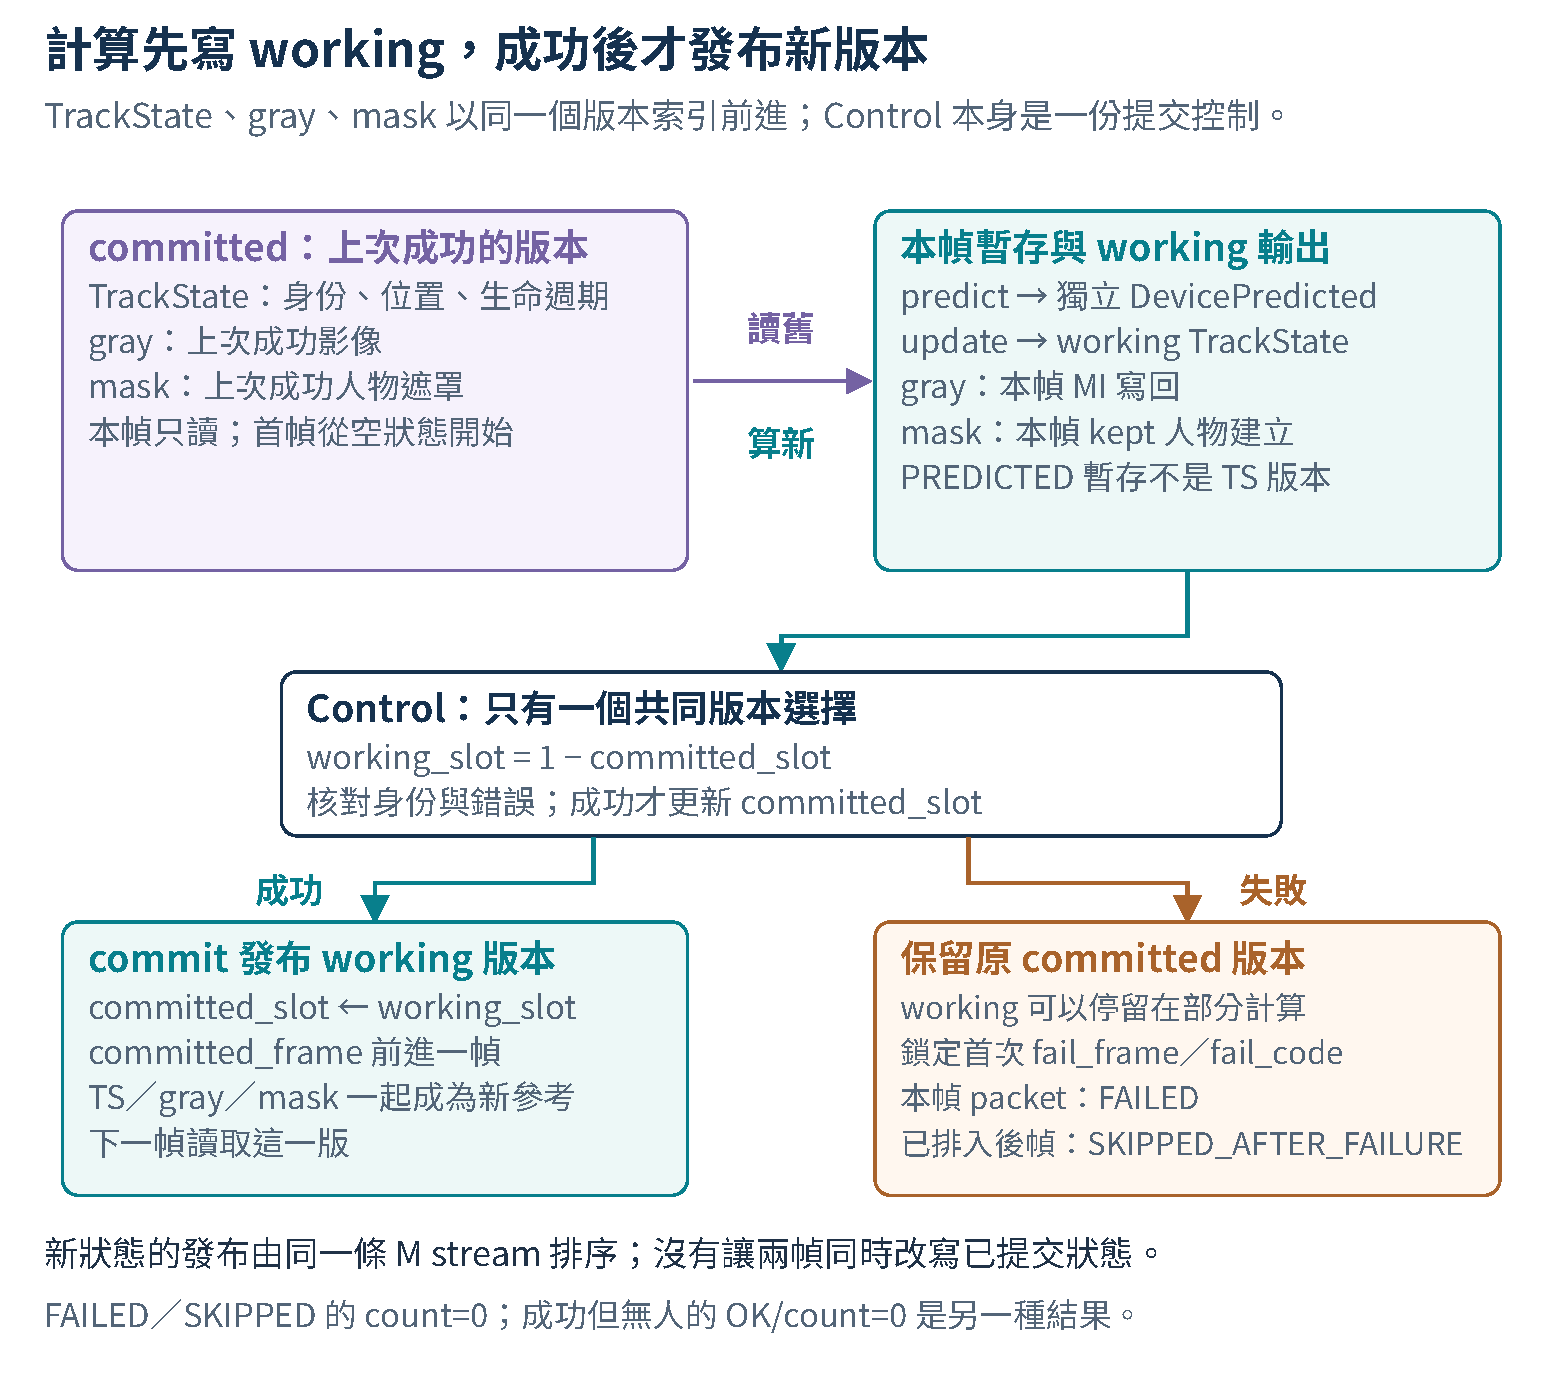
\includegraphics[width=\textwidth,height=130mm,keepaspectratio]{assets/state.pdf}
\caption{讀 committed、寫 working；只有成功 commit 才一起發布新的追蹤與運動參考版本。}
\end{figure}

初始化時 committed\_frame=−1，committed\_slot=1，對應空 TrackState 與無效運動參考。Begin 選 working\_slot=1−committed\_slot；predict 先寫獨立 DevicePredicted 暫存，update 才寫 working TrackState。Gray／mask 寫回也只改工作版本。\cite{state}

{\raggedright \textbf{三種封包狀態。} OK 表示本幀成功提交，count=0 是合法空結果。FAILED 是首次失敗幀；SKIPPED\_\allowbreak AFTER\_\allowbreak FAILURE 是其後已排入幀。後兩者 count=0、保留首次 fail\_frame／fail\_code，不能解讀成成功沒有目標。\par}


自訂計算讀取階段開始前固定的 \code{run_stage}；begin／控制／commit／packet 仍必須執行。函式庫工作可能已排入，仍可寫隔離／working 資料，因此失敗不表示整條 GPU 後續完全不執行。最後成功版本與 slot 歸還依賴都必須保留。\cite{state,flow}

\clearpage
\section{結果回到 CPU 之後，什麼時候才算完成}
TrackingSession 依設定固定採 JPEG、host RGB 或 device video 輸入。兩個 CLI 共用 GPU 追蹤主線，但「收到本幀結果」與「最終 MOT 已完成」是不同時點。

\textbf{D2H 交付小型結果副本。} M stream 依序複製 \code{MotionContext} 56 B 與固定 packet 12,368 B，每幀共 12,424 B，再記錄 done event。前者是受測 ABI 的 struct 大小，後者是序列化 bytes，並非 \code{sizeof(ResultPacket)}。\code{receive()} 等 done、核對 packet 的 epoch／frame，回傳 owned 副本並歸還 host slot，不追加 GPU predict／update。\textbf{Device MotionContext 使用單一重用 buffer；FAILED／SKIPPED 封包附帶的 motion 不保證是新的當幀估計，須先看 packet.status。}\footnote{\path{src/tracking_session.cpp}:479--502；\path{include/saccade/protocol.hpp}:15--18。}

現行 tracker 只輸出 confirmed、age=0 的 observed rows；預設 \code{measurement_box=false}，座標取濾波後 Kalman state。ABI 可表達 predicted rows，不表示目前會輸出 lost tracks。\footnote{\path{cuda/tracking.cu}:449--463；預設設定見 \path{include/saccade/tracking.hpp}。}

\begin{table}[H]
\caption{入口共用追蹤計算，輸出政策不同}
\small
\begin{tabularx}{\textwidth}{@{}>{\raggedright\arraybackslash}p{24mm}>{\raggedright\arraybackslash}X>{\raggedright\arraybackslash}X@{}}
\toprule
環節 & JPEG sequence & 影片／串流 CLI \\
\midrule
輸入 & CPU 讀 JPEG，nvJPEG 交付 GPU RGB & 預設 FFmpeg／NVDEC 交付 device NV12／P010，經 CUDA 色彩轉換 \\
提交／接收 & result ring 滿時先 receive；EOF 後 drain & 每幀 enqueue 後立即 receive、寫出並 flush；預設一格 result ring \\
輸出政策 & \code{v1-mot/1}：首次遇到的 output ID 重編號，EOF 後插值、排序及寫最終 MOT & \code{stream-observations/1}：保留 packet output ID，逐幀輸出，不作序列尾插值 \\
\bottomrule
\end{tabularx}
\end{table}

\textbf{離線補框在 CPU 定稿時做。} \code{SequenceOutput::add()} 收集 packet 全部 rows，不另篩 observed flag。\code{finish()} 預設對至少五筆 rows 的同一輸出 ID，在兩筆 rows 間最多補 35 個缺幀；線性插值 xyxy，補入列 conf=$-1$。writer 轉成 left／top／width／height、取三位小數，不另裁切座標。串流檔案則是逐幀可讀的前綴，正常 EOF／frame-limit 與成功退出才表示要求範圍完成。\footnote{\path{include/saccade/mot_output.hpp}:20--22；\path{src/mot_output.cpp}:16--82；\path{tools/track_stream.cpp}:231--267、349--374。}

\textbf{三個完成邊界：} M 計算／commit 之後還有兩次 D2H；done event 之後還有 \code{receive()} 的 CPU 複製與核對；JPEG 的最終 MOT 還要等 EOF 後 \code{output.finish()} 與寫檔。\code{track_sequence} 的 wall time 停在 drain 完成，排除其後的 close、插值與最終寫檔。\footnote{\path{tools/track_sequence.cpp}:124--148；stream 預設與 flush 見 \path{tools/track_stream.cpp}:84--104、214--216。}

來源 \code{pts_us} 沒有改變 Kalman dt：目前每個解碼幀仍做一次固定步長 predict。即時 flush 亦不代表 fsync 或下游已收到結果。


\clearpage
\section{來源、設定與這篇文章的界線}
本文固定程式基準為 \path{3cbaa518f0dc37d691404e95ed85c0109c81130d}。現行 HR engine SHA-256 為 \path{8292cc233019d08f1b1b6cfbc12f1fe1644f66f2164fd8f50a69b660a7817876}；資料流圖不代表本文重建了 engine，或重新跑過 GPU／品質／sanitizer。

\begin{table}[H]
\caption{要回到實作核對時，可以從這些入口開始}
\small
\begin{tabularx}{\textwidth}{@{}P{27mm}Y@{}}
\toprule
主題 & 專案相對路徑 \\
\midrule
Session 排程 & \path{src/tracking_session.cpp}、\path{include/saccade/tracking_session.hpp} \\
G1／影像版本 & \path{cuda/flow_motion.cu}、\path{include/saccade/flow_motion_cuda.hpp}、\path{docs/TRACKING.md} §20 \\
模型與候選 & \path{include/saccade/model_profile.hpp}、\path{src/head_trt_network.cpp}、\path{cuda/postprocess.cu} \\
追蹤與提交 & \path{cuda/tracking.cu}、\path{cuda/tracking_session.cu}、\path{src/tracking_tail_graph.cpp} \\
封包與輸出 & \path{include/saccade/protocol.hpp}、\path{src/protocol.cpp}、\path{src/mot_output.cpp} \\
入口與輸出政策 & \path{tools/track_sequence.cpp}、\path{tools/track_stream.cpp} \\
本篇來源收據 & 同目錄 \path{sources.json}、\path{contract-audit.json}、\path{figures.json} \\
\bottomrule
\end{tabularx}
\end{table}

\textbf{資料大小的界線。} 表中的 tensor／wire payload 不包含 TensorRT、nvJPEG、NVOF 的私有配置、workspace、pitch padding 或 Graph／driver 成本；不能直接當成完整顯存或實際頻寬。

\textbf{同步與驗證的界線。} 這些依賴描述支援既有受測使用方式。完整 G1 memcheck、原生排隊完整 Graph racecheck、nvJPEG initcheck 等 OPEN／FAIL 仍依原證據保留；圖上的順序與輸出相同不能取代這些驗證。

\begin{thebibliography}{9}
\footnotesize
\bibitem{session} TrackingSession API 與實作，\path{include/saccade/tracking_session.hpp}、\path{src/tracking_session.cpp}。
\bibitem{model} 模型 profile 與 scan head，\path{include/saccade/model_profile.hpp}、\path{src/head_trt_network.cpp}；\path{docs/HEAD_TRT.md}。
\bibitem{preprocess} 前處理實作與數值政策，\path{src/preprocess.cpp}、\path{cuda/resize.cu}；\path{docs/PREPROCESS.md}。
\bibitem{post} 候選與續追，\path{include/saccade/postprocess.hpp}、\path{cuda/postprocess.cu}、\path{cuda/tracking.cu}。
\bibitem{flow} G1 motion 實作與契約，\path{cuda/flow_motion.cu}、\path{docs/TRACKING.md} §20。
\bibitem{state} 提交與固定封包，\path{cuda/tracking_session.cu}、\path{include/saccade/protocol.hpp}、\path{src/protocol.cpp}。
\bibitem{trace} 既有 G1 trace 的可移動重算證據：\path{evidence/report1/2026-11-12-schedule-trace/}。原 capture 為 2026-11-05、乾淨 \code{fae5cb7}，資料與獨立 SQL 核對見其 \path{README.md}、\path{summary.json}、\path{independent-review.json}。
\end{thebibliography}
\end{document}
